\documentclass[10pt,a4paper,fullpage]{article}

\usepackage[utf8]{inputenc}
\usepackage[T1]{fontenc}
\usepackage{amsmath}
\usepackage{amsfonts}
\usepackage{amssymb}
\usepackage{graphicx}
\usepackage{geometry}
\usepackage{array}
\usepackage{multirow}
\usepackage{caption}
\usepackage{booktabs}
\usepackage{titling}

\geometry{a4paper, margin=1in}
\pagenumbering{gobble} 

\newcolumntype{C}[1]{>{\centering\let\newline\\\arraybackslash\hspace{0pt}}m{#1}}

\begin{document}

\title{Pattern Recognition - Exercise 2c (CNN)}
\author{}
\predate{}
\postdate{}
\date{\vspace{-5ex}}
\maketitle


\textbf{Implementation details}
\begin{itemize}
	\item We didn't use a constant learning rate. Instead, the learning rate was decreasing with 10\% from one epoch to another.
	\item We used cross validation with 5 number of folds to determine the pair (number of epochs, learning rate) for which we were able to train the model with the highest accuracy (on the validation set that we extracted from the initial train set). Then, with these 2 values found, we trained the model once again (on the whole train dataset this time) and evaluated it using the test dataset.
	\item For computing the loss we used cross-entropy.
	\item For the optimizer, we chose Stochastic Gradient Descent.
\end{itemize}


\textbf{Testing details}
\begin{itemize}
	\item Number of epochs: 8, 10, 15, 20
	\item Initial learning rate: 0.01, 0.05, 0.08, 0.1, 0.12, 0.13 (we tried larger values than 0.1 too because it's decreasing from one epoch to another)
	\item Batch size: 32
\end{itemize}


\textbf{Results}
\begin{itemize}
	\item Number of epochs: 15
	\item Initial learning rate: 0.13
	\item Accuracy: 98.60\%
\end{itemize}

%[tensor(95.7300), tensor(96.5450), tensor(97.3767), tensor(97.8817), tensor(98.1200), tensor(98.3050), tensor(98.1833), tensor(98.6967), tensor(98.6883), tensor(98.8883), tensor(98.9483), tensor(99.), tensor(99.0883), tensor(99.0117), tensor(99.1883)]
%[tensor(96.3700), tensor(96.7400), tensor(97.3000), tensor(97.7300), tensor(97.9400), tensor(98.0800), tensor(97.7600), tensor(98.3400), tensor(98.3300), tensor(98.5500), tensor(98.4400), tensor(98.4000), tensor(98.5000), tensor(98.3000), tensor(98.6000)]
%[0.19953529501954714, 0.13882767938276133, 0.1137883709291617, 0.09901967648665111, 0.10372261369427045, 0.09636154359529416, 0.09146570273737113, 0.08195805782973767, 0.06428273197263479, 0.06427820384502411, 0.05780567031676571, 0.05749462191462517, 0.055869576928267876, 0.04993066525583466, 0.04732598440771302]
%[0.18591308135986329, 0.1306828811645508, 0.1090241943359375, 0.09892452392578124, 0.1055341064453125, 0.09604759902954102, 0.09663632354736328, 0.08595323333740235, 0.07003974075317383, 0.07019105796813965, 0.06680742149353028, 0.0665325912475586, 0.06515393524169921, 0.06125670204162598, 0.05869334564208984]


%[0.18591308135986329, 0.1306828811645508, 0.1090241943359375, 0.09892452392578124, 0.1055341064453125, 0.09604759902954102, 0.09663632354736328, 0.08595323333740235, 0.07003974075317383, 0.07019105796813965, 0.06680742149353028, 0.0665325912475586, 0.06515393524169921, 0.06125670204162598, 0.05869334564208984]

\vspace{-0.5cm}
\begin{center}
	\begin{tabular}{ r | c | c | c | c }
		\hline
		\multicolumn{1}{c|}{} & \multicolumn{2}{c|}{\textbf{Accuracy}} & \multicolumn{2}{c}{\textbf{Loss}}\\
		\hline
		\textbf{Epoch} & Train Dataset & Test Dataset & Train Dataset & Test Dataset\\
		\hline
		1 & 95.73\% & 96.37\% & 0.1995 & 0.1859 \\
		2 & 96.54\% & 96.74\% & 0.1388 & 0.1306 \\
		3 & 97.37\% & 97.30\% & 0.1137 & 0.1090 \\
		4 & 97.88\% & 97.73\% & 0.0990 & 0.0989 \\
		5 & 98.12\% & 97.94\% & 0.1037 & 0.1055 \\
		6 & 98.30\% & 98.08\% & 0.0963 & 0.0960 \\
		7 & 98.18\% & 97.76\% & 0.0914 & 0.0966 \\
		8 & 98.69\% & 98.34\% & 0.0819 & 0.0859 \\
		9 & 98.68\% & 98.33\% & 0.0642 & 0.0700 \\
		10 & 98.88\% & 98.55\% & 0.0642 & 0.0701 \\
		11 & 98.94\% & 98.44\% & 0.0578 & 0.0668 \\
		12 & 99.00\% & 98.40\% & 0.0574 & 0.0665 \\
		13 & 99.08\% & 98.50\% & 0.0558 & 0.0651 \\
		14 & 99.01\% & 98.30\% & 0.0499 & 0.0612 \\
		15 & 99.18\% & 98.60\% & 0.0473 & 0.0586 \\
		\hline
	\end{tabular}
\end{center}

% From https://timodenk.com/blog/exporting-matplotlib-plots-to-latex/
\begin{figure}
	\begin{center}
%		\input{cnn_model_plot.pgf}
		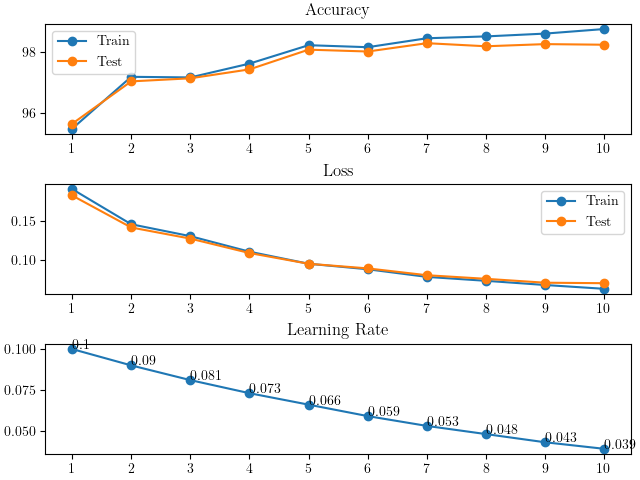
\includegraphics[scale=1]{cnn_model_plot.png}
	\end{center}
%	\caption{A PGF histogram from \texttt{matplotlib}.}
\end{figure}


\end{document}